\chapter{Evaluation}

\textit{In this section I compare the performance of the semi-supervised models on both the MNIST and TCGA datasets, and compare these 
to a fully supervised MLP operating on only the labelled data. I then discuss how these factored into the choices made for a more general
tool. All the results in this section can be replicated using the Python and bash scripts found in the scripts folder}

\section{MNIST}

\subsection{Semi-supervised results}
The MNIST results are important for establishing whether the ladder and M2 models have been correctly implemented, as they should 
achieve close to paper accuracy. It should also give some indication of how the models are expected to perform on the gene expression data.

The MNIST dataset has a designated train and test set, so to obtain the results for this I performed 5-fold cross validation over the 
training set, using 48,000 examples for testing and 12,000 for validation and then computing the accuracy of the model on the 10,000
test samples. Accuracy is computed as the number of datapoints in the test set where the label was correctly predicted divided by the 
total number of datapoints in the test set, given below as a percentage of points correctly classified.
\begin{table}[H]
  \label{tab:mnist_accuracy}
  \small % text size of table content
  \centering % center the table
  \begin{tabular}{R|CCCCC} % alignment of each column data
  \toprule[\heavyrulewidth]\toprule[\heavyrulewidth]
  & \multicolumn{5}{c}{\textbf{Models}}\\
  \shortstack{Number of \\ labelled samples} & \textbf{MLP} & \textbf{SDAE} & \textbf{M1} & \textbf{M2} & \textbf{Ladder} \\ 
  \midrule
  100 & 71.75 \pm 0.82 & 74.86 \pm 0.85 & 49.00 \pm 0.98 & 92.34 \pm 0.52 & 96.64 \pm 0.35\\
  1000 & 88.86 \pm 0.62 & 91.97 \pm 0.53 & 83.44 \pm 0.73 & 96.57 \pm 0.36 & 98.03 \pm 0.27\\
  3000 & 93.88 \pm 0.47 & 95.60 \pm 0.40 & 88.55 \pm 0.62 & 97.19 \pm 0.32 & 98.35 \pm 0.25\\
  \text{All} & 98.41 \pm 0.25 & 98.58 \pm 0.23 & 90.30 \pm 0.58 & 98.45 \pm 0.24 & 98.95 \pm 0.20\\
  \bottomrule[\heavyrulewidth] 
  \end{tabular}
  \caption{MNIST 5-fold cross-validation percentage accuracies} 
\end{table}

\subsubsection{Performance comparisons}
The MLP and SDAE do not have standard accuracies that can be obtained from papers, but the slight performance boost the SDAE provides 
over the MLP when only some of the data is labelled is what was expected.

The results for M1 are much worse than those in the original Kingma paper~\cite{DBLP:journals/corr/KingmaRMW14}, and this is due to the use
of a neural network as the classifier on the latent dimension. This neural network can only use the labelled samples, while the Kingma 
paper uses a transductive support vector machine, which is able to utilise the unlabelled samples in separating the classes. In order to
not overcomplicate the project I decided against implementing a TSVM and so the results are poor. Part of the reason the results are worse 
than even the basic MLP is that the supervised learning cannot update the weights of the VAE. If the VAE is encoding useless information, 
the supervised update steps are unable to prevent this.

The results for M2 are comparable to those in the Kingma paper, and for the 100 labelled samples are actually better, averaging 92.34 
compared to 88.03. I believe that these improvements are due to performing hyperparameter optimisation over the latent dimension of the 
model, whereas the Kingma paper used a fixed latent size of 50.

The ladder results are again comparable, with my implementation averaging 96.64 compared to 98.94 by Rasmus~\cite{DBLP:journals/corr/RasmusVHBR15}
for 100 labelled samples.
The discrepancy is likely due to the slight differences in model structure. I optimise over 1 to 4 hidden layers of fixed size,
while Rasmus uses 5 hidden layers with an overcomplete (1000 neurons) first hidden layer.

\subsection{Saliency}

Saliency maps computed using both normal and guided backpropagation are below, demonstrating how the models learn the important 
sections of the image for classifying.

\begin{figure}[H]
  \centering
  \begin{subfigure}[b]{0.4\linewidth}
    \centering
    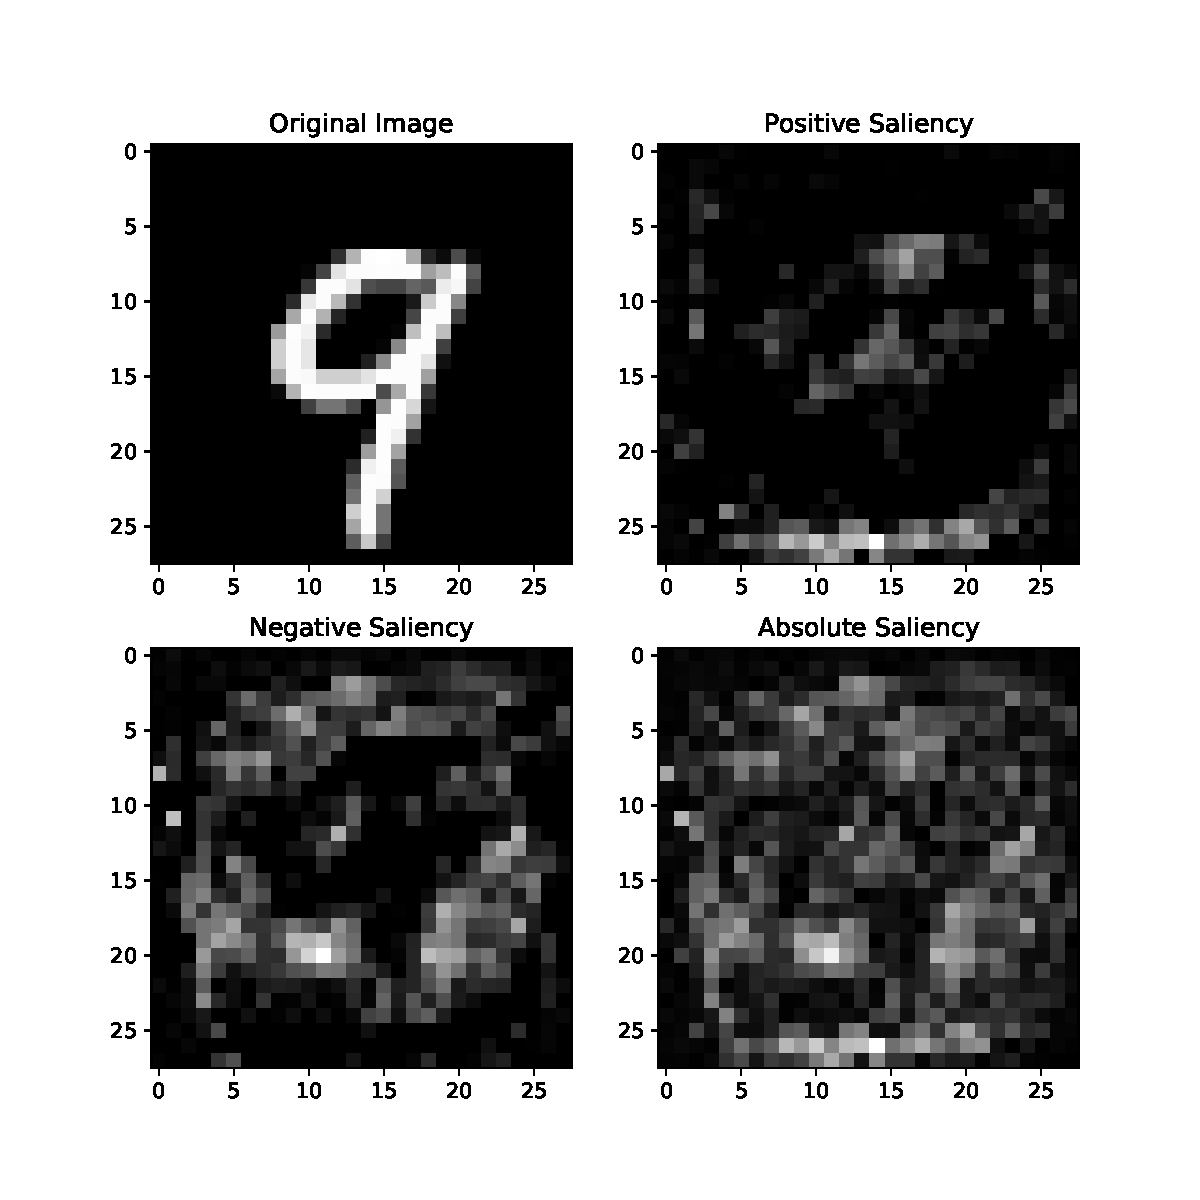
\includegraphics[scale=.25]{figs/vanilla_saliency_maps.pdf}
    \caption{Vanilla saliency}
  \end{subfigure}
  \begin{subfigure}[b]{0.4\linewidth}
    \centering
    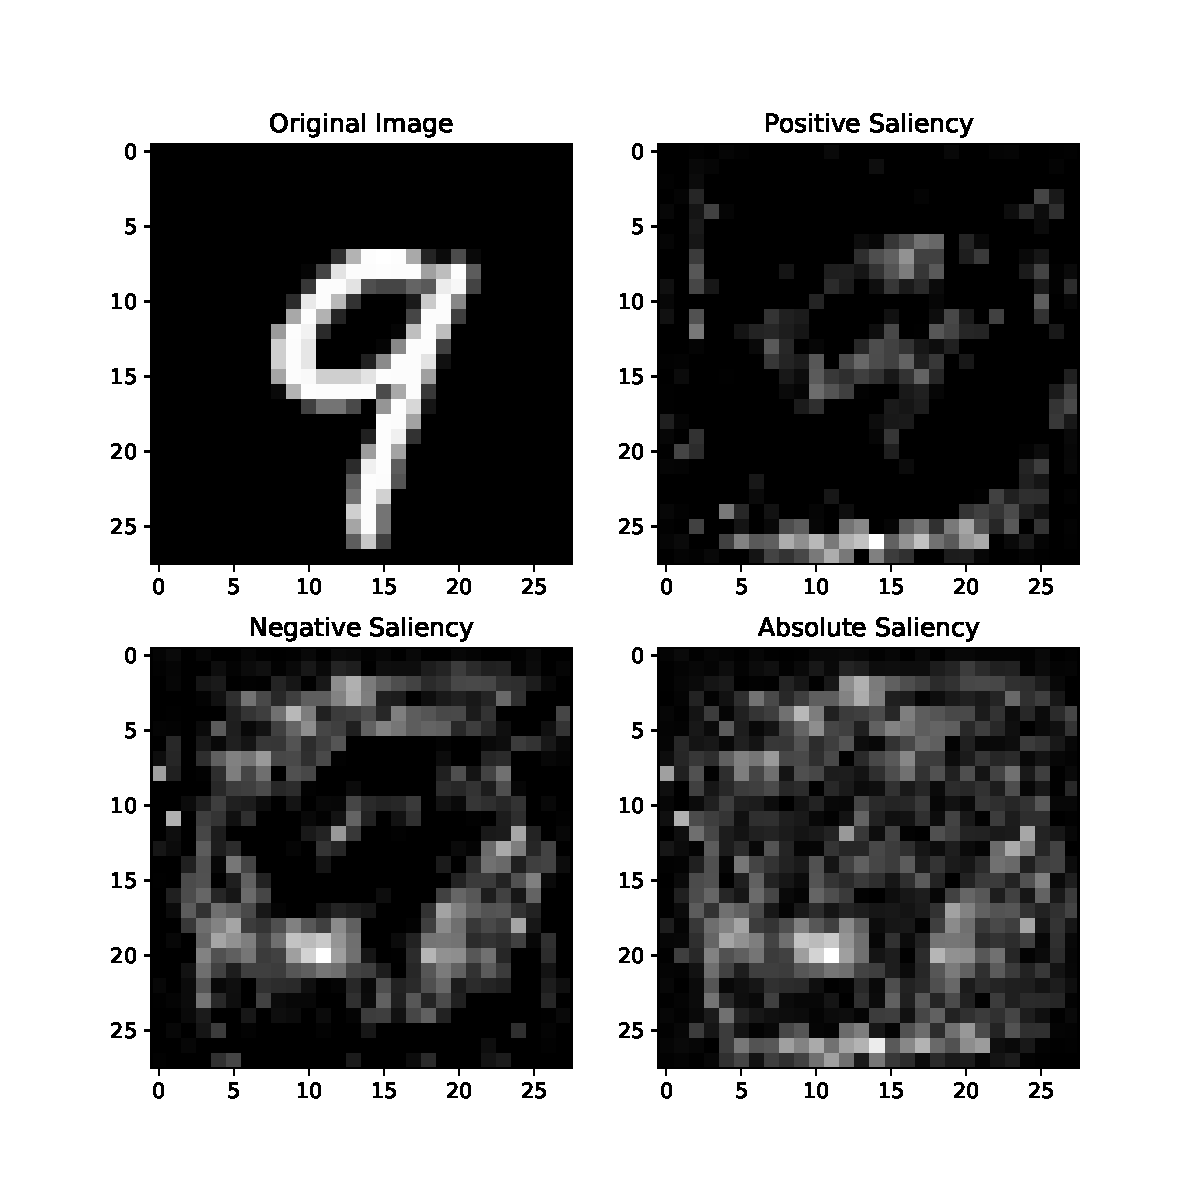
\includegraphics[scale=.25]{figs/guided_saliency_maps.pdf}
    \caption{Guided saliency}
  \end{subfigure}
  \caption{Saliency maps for 9}
  \label{fig:saliency}
\end{figure}

The difference between the two saliency types is subtle, but the guided saliency maps are generally less noisy than the vanilla saliency.
There is a clear outline of the top of a 9 in the positive saliency maps, and the high scoring pixels in the negative saliency maps would transform 
it into an 8 or possibly a 4. In this way these maps allow a user to understand what inputs are important for the network classification.

\section{TCGA results}

\subsection{Missing data} \label{imputation}

As some of the samples in the TCGA dataset are missing expression levels for certain genes I decided to compare the results (using an MLP 
and all of the data as labelled data) of three different techniques for removing the missing values. The first technique was to just drop
all the columns of genes with any missing values, reducing the number of genes from 20,350 to 16,334. The second technique involved 
replacing all the missing gene expression values with zero, and the third involved replacing them with the mean of the expression 
level for all the samples. See table ~\ref{tab:imputation}:
\begin{table}[H]
  \small % text size of table content
  \centering % center the table
  \begin{tabular}{CCC} % alignment of each column data
  \toprule[\heavyrulewidth]\toprule[\heavyrulewidth]
  \textbf{Drop genes} & \textbf{Zero} & \textbf{Mean} \\ 
  \midrule
  95.09 \pm 0.40 & 95.67 \pm 0.38 & 95.81 \pm 0.37 \\
  \bottomrule[\heavyrulewidth] 
  \end{tabular}
  \caption{TCGA data imputation 10-fold cross-validation percentage accuracies}
  \label{tab:imputation} 
\end{table}

Computing a paired t-test helps discern if any one method could be considered better.
\begin{table}[H]
  \label{tab:ttest}
  \small % text size of table content
  \centering % center the table
  \begin{tabular}{CCC} % alignment of each column data
  \toprule[\heavyrulewidth]\toprule[\heavyrulewidth]
  \textbf{Mean/Drop genes} & \textbf{Mean/Zero} & \textbf{Drop genes/Zero} \\ 
  \midrule
  1.723 & 0.543 & -1.753 \\
  \bottomrule[\heavyrulewidth] 
  \end{tabular}
  \caption{t statistics for difference between imputation folds} 
\end{table}

None of these t statistics are statistically significant using a two-tailed t-test with p=0.05, and so we cannot reject the null hypothesis
that all the imputation methods have the same performance. However, dropping the genes makes the least sense, as that way some real data is
lost.

\subsection{Semi-supervised results}

The results in this section were obtained by computing cross-validation as in Section~\ref{part}. All samples with missing data were 
dropped from the dataset to avoid bias due to the imputation type. 

One caveat with these results is that they represent an upper bound on the performance of the models, as a validation set is used that is 
sometimes larger than the number of labelled examples in the training set. This is obviously not feasible in real life, and so the 
results when used in a production setting will likely not be as good. However, this validation set was required for a fair comparison,
as the number of layers and epochs that get the best performance from each model greatly differs from model to model.

\subsubsection{Accuracy}

\begin{table}[H]
  \label{tab:tcga_acc}
  \small % text size of table content
  \centering % center the table
  \begin{tabular}{R|CCCCC} % alignment of each column data
  \toprule[\heavyrulewidth]\toprule[\heavyrulewidth]
  & \multicolumn{5}{c}{\textbf{Models}}\\
  \shortstack{Number of \\ labelled samples} & \textbf{MLP} & \textbf{SDAE} & \textbf{M1} & \textbf{M2} & \textbf{Ladder} \\ 
  \midrule
  100 & 77.54 \pm 0.85 & 78.69 \pm 0.84 & 68.83 \pm 0.95 & \textbf{90.92} \pm 0.59 & 87.56 \pm 0.67\\
  500 & 91.09 \pm 0.58 & 91.32 \pm 0.57 & 91.08 \pm 0.58 & \textbf{93.73} \pm 0.49 & 93.26 \pm 0.51\\
  1000 & 93.02 \pm 0.52 & 93.53 \pm 0.50 & 92.20 \pm 0.55 & 93.90 \pm 0.49 & \textbf{94.08} \pm 0.48\\
  \text{All} & 96.47 \pm 0.37 & 96.13 \pm 0.39 & 93.67 \pm 0.50 & 96.53 \pm 0.37 & \textbf{96.69} \pm 0.37\\
  \bottomrule[\heavyrulewidth] 
  \end{tabular}
  \caption{TCGA 10-fold cross-validation percentage accuracies} 
\end{table}

As can be seen from the results in the table, there is no performance benefit in using the M1 model over the simple MLP, but the accuracy 
achieved nevertheless shows that M1 is probably learning an informative manifold. The SDAE shows a slight performance advantage, but 
clearly performs less well than M2 and the ladder.

The ladder and M2 both show a significant performance advantage over the MLP, and computing a t-test between the three models 
it can show which models perform statistically better with each amount of labelled data. 
\begin{table}[H]
  \label{tab:tcga_ttest}
  \small % text size of table content
  \centering % center the table
  \begin{tabular}{R|CCC} % alignment of each column data
  \toprule[\heavyrulewidth]\toprule[\heavyrulewidth]
  \shortstack{Number of \\ labelled samples} & \textbf{MLP/M2} & \textbf{MLP/Ladder} & \textbf{M2/Ladder} \\ 
  \midrule
  100 & -20.61 & -13.40 & 5.36 \\
  500 & -7.86 & -6.47 & 1.98 \\
  1000 & -2.89 & -4.59 & -1.41 \\
  \text{All} & -0.30 & -2.36 & -1.03 \\
  \bottomrule[\heavyrulewidth] 
  \end{tabular}
  \caption{TCGA 10-fold t-statistics between MLP, ladder and M2} 
\end{table}

The significance threshold for a two fold t-test, using  p=0.05 and 9 degrees of freedom, is 2.26. These results 
show the ladder network significantly outperforming the MLP at every amount of labelled data. The M2 model outperfoms the MLP significantly 
until all the data is labelled. At this point the performance should be almost exactly the same as the MLP, as the training of the 
classifier in the M2 model is only controlled by the supervised cross entropy loss. The ladder is outperformed by the M2 model with 100
labelled samples, but with more labelled samples the difference between them is not statistically significant.

\subsubsection{Matthews correlation coefficient}

Accuracy is not always the best metric to use when evaluating a machine learning model, expecially when the classes in the model are 
imbalanced, as it can mean that predicting just the most populous classes results in good accuracy. For binary classification one of the 
preferred methods is the Matthews correlation coefficient, which is regarded as 
a balanced measure even when the classes are unbalanced because it takes into account the balance ratios of the four possible 
categories~\cite{Chicco2017}. There is a multiclass variant of this 
coefficient that ranges between a minimum value of between $-1$ and $0$
(depending on the distribution) and maximum value $+1$. $+1$ means perfect correlation between the predicted and actual labels. 
This is calculated as below for $k$ classes: 

\begin{align}
  \text{MCC} = \frac{\sum_{k}\sum_{l}\sum_{m} C_{kk}C_{lm} - C_{kl}C_{mk}}{
  \sqrt{
  \sum_{k}(\sum_l C_{kl} )(\sum_{k' | k' \neq k}\sum_{l'} C_{k'l'})
  }
  \sqrt{
  \sum_{k}(\sum_l C_{lk} )(\sum_{k' | k' \neq k}\sum_{l'} C_{l'k'})
  }
  }
\end{align}

Calculating this for M2 and the ladder network gives:
\begin{table}[H]
  \label{tab:mcc}
  \small % text size of table content
  \centering % center the table
  \begin{tabular}{R|CC} % alignment of each column data
  \toprule[\heavyrulewidth]\toprule[\heavyrulewidth]
  \shortstack{Number of \\ labelled samples} & \textbf{M2} & \textbf{Ladder} \\ 
  \midrule
  100 & 0.9041 & 0.8683 \\
  500 & 0.9337 & 0.9286 \\
  1000 & 0.9354 & 0.9372 \\
  \text{All} & 0.9631 & 0.9649\\
  \bottomrule[\heavyrulewidth] 
  \end{tabular}
  \caption{Multiclass Matthews correlation coefficient} 
\end{table}

This is actually not much more informative than the accuracy scores, giving very similar results.

\subsubsection{Confusion matrix}

Viewing the confusion matrix can sometimes give a better insight into where a model is successful and unsuccessful. A confusion
matrix has the actual labels on the y-axis and the predicted labels on the x-axis. Each row represents the instances in an actual class 
while each column represents the instances in a predicted class.

The confusion matrices for the TCGA data are very large due to the large number of classes in the data, and so are included in Appendix~\ref{confusion} 
where they can be viewed in larger size.

Both the ladder and M2 matrices are very similar, and show the same weaknesses. \textit{Rectum adenocarcinoma} 
is misclassified almost 
100\% of the time by both models, as it is a very similar cancer to \textit{colon adenocarcinoma}. 
The other often misclassified cancers include \textit{brain lower grade glioma} and 
\textit{glioblastoma mutliforme}, and \textit{uterine carcinosarcoma} and 
\textit{uterine corpus endometriod carcinoma}. All are similar cancers occuring in similar areas of the body.

The difficulty in classifying these using gene expression is to do with the similarities in gene expression within cells of a certain tissue.
Moreover, the boundary between grades of cancer cannot always be well defined, depending on a range of factors 
including rate of growth and necrosis that can cause the cancer to move between grades.

However, when the number of labelled examples is increased these misclassifications are reduced, with only the rectum and colon adrenocarcinoma 
still significantly misclassifed.

\subsubsection{Ensemble learning} \label{ensemble}

One way of improving the performance of a classification model is combining the classifications of two different models which may have learned
slightly different features and class boundaries. The combination of the models can then lead to an improvement in the accuracy as the 
different features and boundaries can combine to make a better classifier. The simplest way of doing this is to sum the softmax 
output of the different models together. Dividing by the number of models then gives a new probability distribution that is the
average of the previous models. The maximum of this distribution is the predicted label, and if the models have learned complementary
features this will improve accuracy. Combining the M2 and ladder predictions produces the results below:

\begin{table}[H]
  \small % text size of table content
  \centering % center the table
  \begin{tabular}{R|CC|CC} % alignment of each column data
  \toprule[\heavyrulewidth]\toprule[\heavyrulewidth]
  & \multicolumn{2}{c}{\textbf{Ensemble statistics}} & \multicolumn{2}{c}{\textbf{t-test}}\\
  \shortstack{Number of \\ labelled samples} & \textbf{Accuracy} & \textbf{MCC} & \textbf{Ensemble/M2} & \textbf{Ensemble/Ladder}\\ 
  \midrule
  100 & 90.89 \pm 0.59 & 0.9036 & -1.17 & 5.34 \\
  500 & 94.00 \pm 0.49 & 0.9365 & 4.11 & 3.39 \\
  1000 & 94.22 \pm 0.48 & 0.9388 & 3.42 & 1.08 \\
  \text{All} & 96.82 \pm 0.36 & 0.9662 & 2.24 & 0.87 \\
  \bottomrule[\heavyrulewidth] 
  \end{tabular}
  \caption{Ensemble statistics} 
  \label{tab:ensemble}
\end{table}

These results are statistically significant improvements over M2 and the ladder network for different amounts of labelled data.
This combined model performs significantly better than M2 (at p=0.05 level) on all but 100 labelled samples, where it does not 
perform significantly worse. It is significantly better than the ladder network for both 100 and 500 labeled samples. 

It seems that this is the best of both worlds, outperforming the individually best models.

\section{Making a tool} \label{tool}

The information in the previous section informed the choices I made in constructing a tool, found in \texttt{main.py}.

The tool is a simple command line tool where the  only arguments a user provides are the file to load the data 
from, the mode the tool should be in and the name of the folder to save any outputs in.

There are two modes: train and classify. In both the data is first loaded in, and  any missing values are imputed using 
mean-value imputation to avoid losing data.

In train mode the labelled data is first split in two, to perform a very simple 2-fold cross validation to find the best hyperparameters for two 
models, M2 and the ladder. The validation accuracies are also saved to a file called \texttt{accs.csv}, to give the user some indication of
how the model is likely to perform.
Once the hyperparameters have been selected, both models are trained using these parameters on the entire dataset. The models are then 
saved to the output folder.

In classify mode the models are loaded from the specified output folder, and the data is passed through both. The outputs are combined 
as described in Section~\ref{ensemble}, and the results are saved to the outputs folder.

\begin{figure}[H]
  \centering
  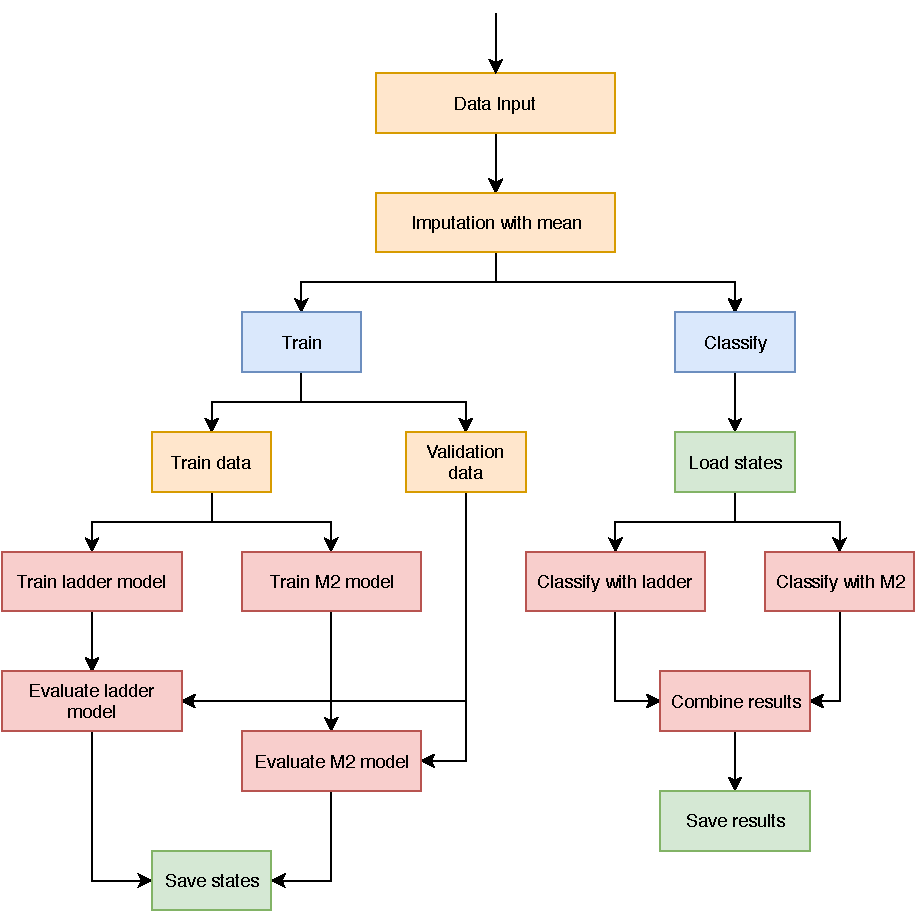
\includegraphics[scale=1]{figs/tool.pdf}
  \caption{Pipeline of the tool}
  \label{fig:pipeline}
\end{figure}